\documentclass[11pt, onecolumn]{article}

% -----------------------
% Packages
% -----------------------
\usepackage{lineno}
\linenumbers

\usepackage{graphicx}	% This package allow you to insert PostScript figures

\usepackage{amsmath} 	% This is a typical math package - it allows you to type certain known math symbols, like exp for expoential 
\usepackage{amssymb} 	% This is a typical math package
\usepackage{amsthm}		% This is a typical math package

\usepackage{color}

\usepackage[utf8]{inputenc}		% can use french characters 
%\usepackage[latin1]{inputenc}

\usepackage{hyperref}

\usepackage{setspace}	% double-spaced text
\doublespacing

\usepackage{apacite}	% To use APA style citation

\usepackage[margin=1in]{geometry} % 1-inch margin around document

\usepackage{enumitem}

\usepackage{array}
\usepackage{booktabs}

\usepackage{xcolor}   % textcolor
% -----------------------


% -----------------------
% Margins
% -----------------------
\setlength{\parindent}{0.6cm}	% indent paragraph by this much

\setlength{\parskip}{0.1cm}	% space between paragraphs
% -----------------------


% -----------------------
% Bibliography
% -----------------------
\bibliographystyle{apacite}		% Style of bibliography presentation
% -----------------------


% Notes/
% \'{e} = é
% \'{e} = è

%\title{}	% the document title
%\author{}
%\date{}

% --------------------- end of the preamble ---------------------------





%----------------------------------------------------------------------------------------

\begin{document}

%------------------------------------------------
\begin{abstract}   % *** Abstract word limit is 250 words maximum ***
%------------------------------------------------
{\bf Objective:}
A comprehensive ergonomics study on Spatial Disorientation (SD) in aviation was performed to demonstrate that a generalized SD perception dataset, measuring perceptual joystick response in different vestibular stimulation contexts, can be created using motion detection experimental methods.  Machine learning modeling (ML) recommendations for predicting SD were established, such that SD researchers can directly apply these modeling techniques to real flight data.

{\bf Background}:
In aeronautics, SD includes situations in which the aviator fails to perceive correctly aircraft attitude, position or motion. SD is often quantified in terms of task and accident use-cases, making it difficult to develop a generalized and fundamental understanding of the occurrence of SD and viable solutions.

{\bf Method:}
Using motion detection experimental design methodologies, a vestibular whole-body rotational and translational compensatory tracking task was employed to investigate SD perceptual joystick response in a naturalistic flight context.  A generalized SD dataset was created from these experiments, whereupon five combinations of key ML modeling parameters were evaluated using prediction accuracy and ROC-AUC; modeling parameters included number of features, eight model types, dataset conditions, feature type, and semi-supervised label type.

{\bf Results:}
The perceptual SD dataset was statistically proven to be representative of human motion detection behavior.  Thus, the simulation environment coupled with motion detection experimental methods was sufficient to generate realistic piloting responses. ML modeling comparison analysis demonstrated that SD can be predicted using joystick motion derived features and give detailed recommendations for the five key ML modeling parameters. Specifically, the number of features per model did not influence model prediction, implying that a single joystick derived feature is sufficient to predict SD.  Moreover, decision tree models produced more accurate SD prediction models than other optimization based models when using simple joystick motion features.  Specialized models per experimental condition did not outperform models where all the data was used for decision tree models.  However, for optimization based models some specialized models predicted better than models in which all the data was used, implying that lower data variability is important for SD prediction using optimization based models.  Feature importance analysis revealed that decision tree models perform best using constant natural frequency features, and optimization based model feature importance identified more temporal features as being important than constant natural frequency features.  Thus, if a simple and stationary SD model is needed, that relies on modal patterns, decision tree models using simplistic joystick derived features are sufficient.  However, if a more complex time dependent SD model is needed, that relies on data trends, optimization based models using more complex joystick derived features are an ideal option.  Binary semi-supervised SD label construction resulted in better predicting models than multi-label construction, in particular the binary label that defined SD by overall correctness produced more accurate prediction models than the label based on initial correctness.  Thus, it is best to define some performance mistakes as non-SD and major performance mistakes as SD; this result confirms the existing definition of SD.

{\bf Conclusion:}
Perceived motion disorientation can be quantified and predicted based on task relevant behavior (e.g., joystick).

{\bf Application:}
These measures can be used to monitor the occurrence of SD, thus understanding the cause, and evaluate the effectiveness of SD solutions. 

\vspace{0.1cm}
\noindent
{\bf Keywords:} aviation, spatial disorientation, vestibular, perception, joystick, machine learning. 
%Up to 5 keywords (exclude words that already appear in the title)
\end{abstract}

%------------------------------------------------
% Précis: a 50-word description (in 1–3 sentences) of the manuscript, which will appear in the Table of Contents below the title and authorship information
%------------------------------------------------
\vspace{0.1cm}
\noindent
{\bf Précis:}\\  % Exactly 50 words
A comprehensive ergonomics study on Spatial Disorientation (SD) in aviation, that simulated SD in a naturalistic piloting context and predicted the occurrence of SD using perceptual joystick responses; motion detection experimental design methodologies and machine learning techniques were used. 


\section{Introduction}
SD, in aviation, is the failure to perceive orientation, position, or movement. It is caused by multiple factors including environmental references and conditions, experience, and stress.  There are diverse types of SD symptoms, ranging from confusion to physical sickness, and currently there is no proven method or solution to prevent it (\cite{Bles_2008_SD}; \cite{Gibb_2010_Aviation}; \cite{Perdriel_1980_SD}; \cite{Previc_2004_Spatial}; \cite{Newman_2007_SD}).  International studies on the frequency and severity of SD accidents show that the cause of $6-32\%$ of major accidents are due to SD, similarly $15-26\%$ of fatal accidents are a result of SD (\cite{Newman_2007_SD}).  Recovery from SD is strongly connected to the pilot's awareness of the situation, and his/her ability to perform corrective control, despite the disorientation, to maintain aerodynamic stability; $80\%$ and $20\%$ of SD incidents are caused by unrecognized and recognized situations respectively (\cite{Bles_2008_SD}).  Currently, SD is treated by educating pilots of the signs and symptoms of SD, and instructing them to fly below the physiological thresholds of the human vestibular system.  Treating SD has been challenging because SD is often defined with respect to a specific aeronautical context. SD definitions focus on flight performance errors but seldom include context independent behavior, perceptual, or physiological trends.  Due to the fact that SD is studied case-by-case in an aeronautical context, there is little general understanding of the onset of SD and orientation, position, or movement perception with respect to environmental references.  It would be of interest to study SD using a motion detection experimental paradigm, measuring SD in a general context with respect to whole-body orientation, position, speed, and perceptual feedback.  And, ultimately outlining a general framework for modeling and predicting the occurrence of SD based on perceptual feedback.

Vibrations or motion, measured by the human vestibular system, contain important information about the environment and our orientation and position with respect to the environment.  Motion detection is the act of discerning self-motion with respect to a reference in the environment (\cite{Chaudhuri_2013_Wholebody}).  Human motion detection and perception is quantified, by stimulating the vestibular system systematically, via different vibrational and motion experimental paradigms (\cite{Angelaki_2008_Vestibular}). Initially, motion detection was quantified by observing at which directions and speeds, angular or linear, humans could perceive self-motion.  Experimental paradigms included the usage of different experimental conditions such as, acceleration amplitude, trajectory of stimuli, sequence and exposure time of movement and non-movement events, movement direction with respect to the orientation of the head, whole-body stimulation (\cite{Melvill_1978_Vertical}).  Recent motion perception research has adopted robotic simulation tools and standardized experimental paradigms, including a greater range of motion test frequencies, allowing for more precise and consistent motion detection boundaries for a large variety of perceptual situations.  Additionally, vestibular motion perception studies investigate context-driven parameters, such as: 1) stimuli direction, rate, and acceleration, 2) vestibular dysfunction vs control detection, 3) orientation and/or movement of the user's body during exposure to stimuli, 4) expertise vs novice detection, 5) user age.  Depending on the context parameters and the stimuli trajectory, the vestibular-proprioceptive system detects motion differently and thus behavioral responses are different (\cite{Soyka_2011_Predicting}; \cite{Valko_2012_Vestibular}; \cite{Hartmann_2014_Direction}; \cite{BermudezRey_2016_Vestibular}; \cite{Karmali_2017_Multivariate}).  For SD applications, the observed values where humans could not perceive correct self-motion, called vestibular thresholds, were used as an indicator to be aware of SD (\cite{Gillingham_1993_Spatial}; \cite{Previc_2004_Spatial}).  However, it remains uncertain how to reliably use thresholds to assist with SD in a functional aviation context.

In an online flight context, it is more accurate to predict states of disorientation from modeled physiological or movement signatures than using vestibular thresholds.  Thus, instead of applying perceptual threshold values from motion detection research to SD research, as was done in the past within aviation, SD researchers are beginning to conduct motion detection experiments using realistic flight scenarios.  For instance, directional perception was investigated in a realistic helicopter task where participants were asked to point towards the sky to demonstrate a non-SD state (\cite{Cheung_2000_Disorientation}).  Similarly, continuous heading detection was investigated using a compensatory task such that perceived heading was measured with respect to a remembered target (\cite{Sargent_2008_Disorientation}).  Most recently, the individual and interactive influence of optical and gravito-inertial stimuli during simulated Low-Altitude Flight demonstrated the importance of sensory integration effects of on height perception (\cite{Denquin_2021_LAF}).  These applied studies are useful and give insightful information about motion perception in realistic contexts.  There is a need for more psychophysical SD motion perception studies using an ergonomics approach, where the results can be generalized and directly used in the field of aviation.

In this study, we investigate SD by using : 1) motion perception experimental methods to create a generalized SD occurrence dataset containing a perceptual feedback measure, 2) statistical and machine learning methods to identify optimal modeling parameters for predicting SD.  During the dataset creation phase, we used existing motion detection experimental design methodologies, and designed a generalized motion detection experiment.  A vestibular whole-body compensatory task in darkness was used to produce realistic motion cues that a pilot might experience, where motion detection behavior was recorded via joystick movements.  Two experiments were conducted, a rotational and translational motion detection task.  The rotational and translational experiments administered angular and linear whole-body stimulation, around and along the 3 Cartesian coordinate frame axes, respectively.  Participants were given randomized combinations of three parameters that created the angular or linear motion stimuli: axis, direction along the axis, and speed.  Similar to recent motion perception experimentation a motion simulation system was used to administer whole-body stimulation.  The goal of the work in phase 1 was to create a realistic and diverse dataset of perceptual joystick motion with respect to the occurrence of SD.  The motivation of the dataset creation phase was not to identify vestibular thresholds and report corresponding behavior, but to recreate realistic flight response data in a controlled manner such that states of disorientation could be modeled.  It was necessary to first recreate a motion detection experiment based on previous research before SD could be investigated and modeled, because there were no public datasets of a naturalistic piloting task that denoted the occurrence of SD while containing a perceptual feedback measure.  Despite the advent of public datasets, such as Google Cloud and Kaggle, psychophysical experimental data for a specific context are rare or unavailable.  Next, using the generalized SD dataset, machine learning methods were chosen for SD modeling because their reliable and effective predictive capabilities (\cite{Burkov_2019_ML}).  During the comprehensive modeling parameter search phase, we 1) categorized participant response into 4 profiles, 2) created 3 semi-supervised labels from the profiles for identifying SD-state, 3) created 6 unique features from the perceptual joystick feedback measure, 4) compared test set prediction accuracy and ROC-AUC for five key modeling parameters: number of features, 8 model types, dataset conditions, feature type, semi-supervised label type.  Machine learning modeling parameter combinations were identified for accurate prediction of SD.  The goal of phase 2 was to create a machine learning model parameter selection guide for SD prediction, such that SD researchers in aviation can readily use these proven parameters with real flight data.  Finally, the relationship between physical sickness symptoms and motion disorientation were investigated to identify potential physical markers for SD; physical sickness was quantified using a generalized disorientation test for humans called the Simulator Sickness Questionnaire (SSQ) (\cite{Kennedy_1993_Simulator}; \cite{Bouchard_2007_SimulatorSickness}).  We hypothesized that participants who correctly detected motion, implying they do not have SD, will additionally not have physical sickness.



\section{Methods}
The rotational and translational SD motion detection experiments were identically designed such that the resulting SD dataset would be in a standard format.  The following experimental parameters were the same for both experiments: experimental stimuli conditions, number of randomized trials per experiment, timeline of experimental events per trial, experimental protocol, motion simulation system.  The classification experiments required that five key modeling parameters be evaluate: number of features, model type, dataset conditions, feature type, semi-supervised label type. Model, feature, and semi-supervised label type were defined using human movement and SD domain specific information.

\subsection{Motion detection experiment}
In order to create a diverse dataset of vestibular and proprioceptive SD response, perceptual response was measured using a 3x3 block design testing a randomized combination of angular or linear axis motion, axial direction, and speed.  32 total participants participated, in both experiments, receiving the same experimental instructions and protocol while using the motion simulator.

\subsubsection{Experimental design and timeline events}
The axis experimental condition had three parameters, cabin movements for rotation were roll (RO), pitch (PI), and yaw (YA), and translation included left/right (LR), forward/backward (FB), and up/down (UD).  In addition, minuscule sinusoidal vibrational noise, 1-2cm in amplitude, was added to the non-stimulated axes to mask the sound of the motor for the selected stimulus.  Due to the fact that vibrational noise was present, participants were exposed to a more realistic aviation environment.  Furthermore, the additional vibration helped to reduce movement detection thresholds such that the task was realistically challenging (\cite{Chaudhuri_2013_Wholebody}).  The axial direction experimental condition had two parameters denoting positive and negative direction.  Figure 1A depicts both axis and axial direction convention for both rotational and translational experiments.  Finally, the speed experimental condition had two parameters, a slow near sub-threshold (sub) speed where motion is difficult to detect and a fast near supra-threshold (sup) speed where motion detection is apparent.  In motion detection literature, our speed parameters are known as motion detection thresholds measured in terms of frequency, using deg/s or cm/s depending on whether the stimulus motion is in rotation or translation respectively.  The speed parameters required special selection such that values would be in alignment with motion detection thresholds and accommodate the motion constraints of the simulation system.  For both rotational and translation experiments, a range of sub and sup speed values were selected from motion detection literature (\cite{Previc_2004_Spatial}; \cite{Melvill_1978_Vertical}; \cite{Hartmann_2014_Direction}).  A calibration phase was conducted with 23 naive participants, where the literature speed values were tested using the motion simulator system.  Calibration phase participant’s sat naturally in the simulator and verbally reported which direction they believed that they were moving directly after randomized motion stimulation.  For the rotational experiment, the chosen sub and sup speed that reported the largest number of correct responses was 0.5 Hz (deg/s) and 1.25 Hz (deg/s) respectively.  Similarly for the translational experiment, the chosen sub and sup speed was 3.75 Hz (cm/s) and 15 Hz (cm/s) respectively.  Method and procedure for threshold selection are detailed in Supplementary Materials.

% -------------------- Figure 1 --------------------
% \begin{figure}[ht]
% \begin{center}
% 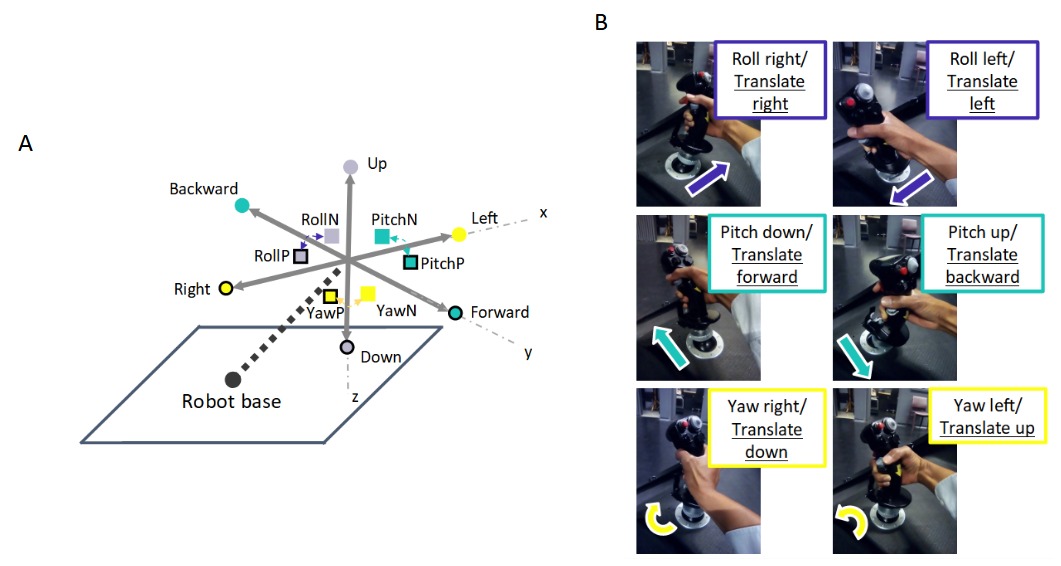
\includegraphics[width=0.9\linewidth]{Figure1_final.png}
% \end{center}
% \caption{The grey Cartesian coordinate frame in Figure 1A represents the simulator cabin, the cabin could move in both rotation (RO, PI, YA) and translation (LR, FB, UD) via the input stimulus and/or participant control. The black outlined squares and circles in Figure 1A denote positive directional movement (RollP, PitchP, YawP, Right, Forward, Down), where squares and circles correspond to rotational and translation movement respectively. Non-outlined squares and circles indicate negative directional movement (RollN, PitchN, YawN, Left, Backward, Up).  Figure 1B shows the mapping of participant’s joystick movements to the cabin movement.}
% \label{Figure1_final}
% \end{figure}
% -------------------- 

A single trial was composed of four different phases, as denoted by the timeline in Figure 2, where participants were tasked to respond to specific visual and vestibular stimuli per phase.  During both phase A and B, participants could move the simulator using the joystick in any of the rotational or translational axes to counteract the perturbation. 

% -------------------- Figure 2 --------------------
% \begin{figure}[ht]
% \begin{center}
% 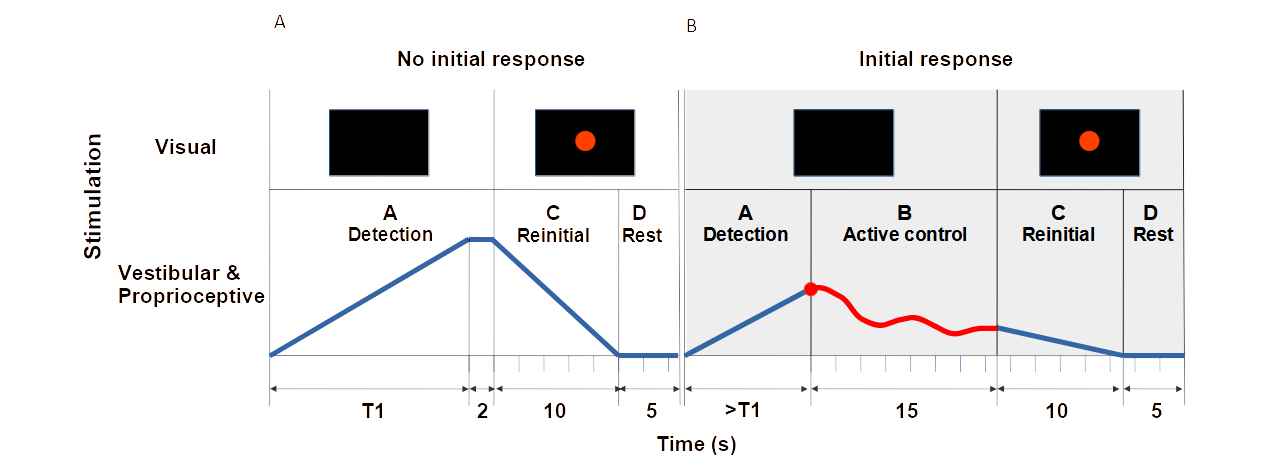
\includegraphics[width=0.9\linewidth]{timeline.png}
% \end{center}
% \caption{The experimental event timeline per trial consisted of four phases:  (A Detection) motion stimulation of the cabin using a smoothed ramp forcing function and participant initial detection, (B Active control) participant active control, (C Reinitialization) cabin reinitialization to the initial orientation or position, (D Rest) cabin and participant at rest.  Visual and vestibular stimulation was given during each phase.  The blue and red lines denote the position-based trajectory of the cabin simulator along one axis per trial. Specifically, the blue line denotes automatic robotic movement, and the red line denotes the stimulus plus the participant’s movements to compensate the perturbation.  T1 denotes the maximum allowed stimulation time per trial with respect to each axis and speed, if initial detection was not made within T1s the experimental phases followed as depicted in A.  If the joystick was moved within T1s, an initial response was registered and experimental phases occured as depicted in B.}
% \label{timeline}
% \end{figure}
% -------------------- 

\begin{itemize}
\item Phase A Detection:  A smoothed ramp forcing function, where the rate of displacement was unknown to the participants, slowly and continuously perturbed one of the three rotational or translational axes of the simulator cabin at a sub or sup rate.  The acceleration profile was the derivative of the position trajectory shown as the blue and red lines in Figure 2.  During phase A participants were tasked to perform "initial detection", which consisted of identifying the axis and direction of the felt perturbation and manipulating an aviation joystick (Thrustmaster Hotas Warthog joystick), shown in Figure 1B, in the opposite direction of the stimuli.  Participants had 15-20s to detect motion depending on the condition, denoted by T1 in Figure 2, which corresponded to the cabin reaching the maximum allowed cabin displacement.  T1 was different for every axis and experiment because sub and sup rates were different for each experiment and the physical cabin displacement range was different for each axis.  In particular, the rotational experiment had slightly longer stimulation times than the translational experiment because the sub and sup rates were slower and the available cabin displacement in the RO, PI, YA orientations were larger than the available translational displacement ranges.  If participants did not respond within T1s during phase A, the cabin automatically displaced along one of the three axes as the ramp function increased until it reached T1s, where upon the ramp function maintained a zero slope causing the cabin to remain stationary for 2s.
\item Phase B Active control: If participants responded within T1 seconds during phase A, phase B active control began and they had 15s to maintain the simulator orientation or position stably at the initial location by counteracting the perturbation.  No visual stimulation was present, thus participants could only rely upon vestibular and proprioceptive cues.
\item Phase C Reintialization: A red dot appeared on the screen instructing participants to release the joystick and rest, while the cabin automatically returned to the initial starting location in 10s. 
\item Phase D Rest: The cabin remained stationary at the starting location for 5s in order to avoid possible over stimulation or after effects.
\end{itemize}

Figure 2 shows two trajectories, when the participant detected and did not respond, demonstrating 
experimental phases and trial length were dependent upon participant response.  The shortest and longest length trial was approximately 32s and 50s respectively.  The shortest length trial would occur if T1=15s and the participant immediately responded (2s+15s+10s+5s) or did not respond  (T1=15s+2s+10s+5s), the longest length trial would occur if T1=20s where the participant responded just before T1 equaled 20s (19.9s+15s+10s+5s).

Both experiments administered 42 trials, 12 familiarization practice and 30 experimental trials.  During the familiarization practice phase, unique experimental condition combinations were given where each of the 3 axes were stimulated in negative or positive directions at sub or sup speeds.  Similarly, the experimental phase consisted of 30 randomized trials, such that 15 trials with unique experimental conditions were repeated twice; 5 direction-speed conditions (negative sup, negative sub, no-movement, positive sup, positive sub) for each of the 3 axes (RO/LR, PI/FB, YA/UD).  No-movement trials were included as sham trials to encourage participants to remain active.

\subsubsection{Participants}
18 and 14 healthy volunteers with normal or corrected vision, and no particular flight experience performed the rotational and translational near sub-threshold tasks (males and females, $32\pm10$ SD years old): 4 of the 32 participants reported having novice time-limited (45 minutes, 2 hours, 40 hours, 45 hours) piloting experiences. 4 of the 18 rotational and 4 of the 14 translational participants were over the age of 40. The participants that performed the rotational experiment were not the same as participants that performed the translational experiment. Therefore, there were no confounds due to experimental ordering, learning, carryover, or fatigue. The same participant population, university students and personal, were used for both experiments therefore it is likely that both experimental populations were similar. 

\subsubsection{Participants}
The experiment took approximately 90 minutes and consisted of four sections: (1) arrival/ questionnaires/ instruction, (2) familiarization, (3) active control of rotational or translational stimulation, (4) questionnaire/discussion.  After describing the experimental task and the completion of the questionnaires, participants were securely installed, using the safety harness and communication headphones, as shown in Figure 3A. They were asked to moderately move the joystick in one axis direction at a time while compensating the unknown perturbation.  Participants were reminded to maintain the cabin at the initial trial position or orientation by compensating the motion stimulus.  The reaction time and/or strategy that participants adopted were chosen by the participants, no instruction was given regarding response quickness or accuracy.  In order to replicate a realistic flight scenario, participants were free to move their head and body, looking and/or fixating where they wished, as long as it did not interfere with the task.  Once the participant was installed in the cabin, the cabin door was closed and all communication between the participant and experimenter were performed via a camera interface system which facilitated two-way auditory visual communication. The physical well-being of the participants were monitored, the experiment ended if participants showed signs of physical illness. 

% -------------------- Figure 3 --------------------
% \begin{figure}[ht]
% \begin{center}
% 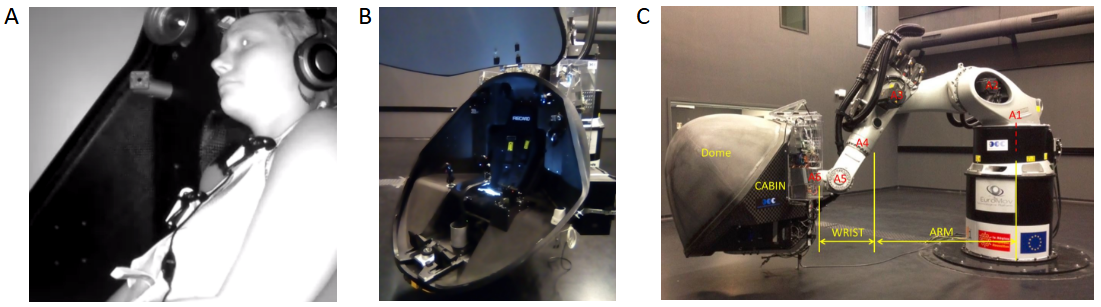
\includegraphics[width=0.9\linewidth]{Figure2_exp_protocol_simulator.png}
% \end{center}
% \caption{Motion simulator apparatus and installation.  A and B show the experimental simulator cabin with and without a seated participant.  C shows an exterior view of the six-axis KUKA motion simulator, consisting of the participant cabin and the robotic arm.}
% \label{Figure2_exp_protocol_simulator}
% \end{figure}
% -------------------- 

The motion simulation system, that provided sensory stimulation, consisted of a 6-degree-of-freedom position controlled KUKA-based motion simulator system (KR 500-3 MT adapted by BEC GmbH motion simulators, KUKA Roboter GmbH, Germany) and a closed-network of three independent workstations (\cite{Denquin_2021_LAF}; \cite{Landrieu_2017_Timetocollision}; \cite{Bellmann_2011_DLR}).  Figures 3B and 3C show the interior and exterior of the simulation system, data was transferred between the KUKA and Workstations at 250Hz on a private UDP protocol network.  Workstation 1 and 3 were located in another room, where workstation 1 generated motion for the KUKA robot using a Matlab/Simulink control interface program (MATLAB and Simulink Toolbox Release 2009, The MathWorks, Inc., Natick, Massachusetts, USA).  Workstation 2 was fixed to the simulator cabin, it administered the red dot or black visual screen and registered joystick motion.  Workstation 3, using Labview, served as the experimenter user control interface to start and stop the experiment, and collect experimental data without causing information delays between the workstations.



\section{Analysis}
As previously mentioned, the goal of this study was to create a realistic flight dataset of moments of disorientation and non-disorientation measured by joystick motion, and then identify the best methods for predicting SD using machine learning methods.  Performed analysis methodologies were: 1) verifying the correctness and authenticity of the dataset in a categorical manner, 2) evaluating ML modeling parameters for SD classification using three metrics, 3) correlating physical with perceptual disorientation to confirm if other possible measures besides joystick could convey markers for the occurrence of human SD-state.  Python was used for all analyses, using packages numpy, pandas, scipy, sklearn, seaborn/plotly/matplotlib  (Python 3.9, Python Software Foundation, Fredericksburg, Virginia, USA). 

\subsection{Verification of simulation dataset: correctness of data collection}
All 42 trials, familiarization and experimental trials, were used in order to maximize data usage.  Simulator system motion and participant joystick responses were down-sampled from 250Hz to 10Hz for data analyses, such that only relevant human motor movements were considered; literature has shown that human hand and arm movements do not exceed frequencies of 10Hz (\cite{Shadmehr_2004_Computational}).

Next, data standardization pre-processing analysis was performed to ensure that the experiment functioned correctly for all trials and participants.  In order to conform with the experimental design, joystick responses needed to influence the correct cabin axes within a window of a few seconds.  Trials where the joystick response did not follow the experimental design due to real-time system delays were removed; $40\%$ of rotational and $50\%$ of translational trial data was removed from the analysis.  Data standardization was the only step that removed trial data, trials that passed data standardization were used in data analysis even if it was a familiarization trial where participants had less practice.

See the Supplementary materials section for the steps used to standardize the data.  Considering the real-time functional programming and communication complexity of the motion simulator system, it was not alarming that many trials were removed due to small errors caused by system delays.  Small functional delays originated from Simulink's block execution priority and available system resources to process the real-time tasks.

\subsection{Categorization of response}
Detection of correct stimuli was categorized into ten possible categories based on the selection of axis and axial direction.  See the Supplementary materials section for a detailed flow chart of the possible participant choices based on response movement.

The ten detection performance profiles were reduced to four categories: 
\begin{itemize}
\item Initial Correct axis $\&$ direction : trials where the first response was with the correct axis and direction (IC : Category 1)
\item Eventually Correct axis or direction: trials where the first response was with an incorrect axis or direction  (EC : Category 2, 4, 5)
\item Never Correct: trials where participants acted on the joystick but never found the correct axis and/or direction (NC : Category 3, 6, 7)
\item No response: trials in which participants did not respond (NR : Category 9).
\end{itemize}

Categories 8 and 10 corresponded with No-movement sham trials, and were not used in the analysis.


\subsection{Verification of simulation dataset: motion detection behavior and performance summary}
Normalized response count and Reaction Time (RT) per detection performance category was quantified per axis and speed condition.  Normalized response count was the adjusted count per response category, with respect to the given number of trials multiplied by participants; the total trial count per participant was 36 not including sham trials.  The total trial count per participant was adjusted to 36 such that interpretation of results would be coherent with the experimental design.  Participants had less total trials than 36 trials because trials that did not follow the experimental design were removed during the data standardization step mentioned in subsection 3.1.  RT was the time required before the participant found the correct axis and direction.  The $95\%$ confidence interval per axis was calculated to determine which detection performance categories were significant; detection performance categories above the lower confidence interval were evaluated further.  Significant and corresponding detection performance categories were compared per speed and axis.  

The Kolmogorov-Smirnov test (kstest) was used to evaluate whether to use a parametric or non-parametric two-sample comparison test for within and across axis comparisons.  All kstest evaluations resulted in non-parametric distributions thus only non-parametric tests were used.  Three non-parametric tests were used to evaluate comparisons, using Bonferroni correction: Wilcoxon signed rank distribution test, Wilcoxon sum rank distribution test, Barlett distribution variance test.  Uneven two-sample data vectors were compared using the Wilcoxon sum rank test and the Barlett test.  However, the Wilcoxon signed rank test required that equal length vectors be compared, thus shorter length vectors were padded with nan values.
A participant detection performance rank score was created in order to understand how well participants performed with respect to perfect performance and with respect to each other.  The performance rank score was calculated per subject across trials, evaluating how many times the participant achieved a certain detection category: 
(IC count)*2 + (EC count)*1 + (NC count)*0 + (NR count)*0.

IC performance was the desired behavior for the task so a weight of 2 was given to each IC trial.  EC was also desired task behavior because participants were able to eventually find the correct axis and direction, however mistakes were made, thus a weight of one was given to each EC trial.  NC and NR performance trials were not the desired task behavior so they were given no credit.  The maximum achievable rank score was 72, if the participant performed IC detection for all 36 stimuli trials; as a reminder each participant received 42 trials and 6 trials were no stimuli sham trials.  Finally, the participants were divided into 3 categories, by using 1 standard deviation from the mean rank score as a margin for average performance, to summarize performance with respect to each experiment. Best performers were greater than the mean rank score plus 1 standard deviation, and worst performers were less than the mean rank score minus 1 standard deviation.

\subsection{Classification model evaluation}
Average 5-fold cross validation test prediction accuracy and Receiver Operating Characteristic Area Under the Curve (ROC-AUC) measures were used to evaluate ML model performance.  Accuracy measures the true positive and negative count over the total number of samples, (TP+TN)/(TP + TN + FP + FN).  Accuracy only gives information about how well the model approves data, but not about how well the model rejects data.  Therefore, a common measure called ROC-AUC is used to evaluate both classification acceptance and rejection performance.  ROC-AUC is the area under the false positive rate FPR=FP/(FP+TN) versus the true positive rate TPR=TP(TP+FN) (\cite{Burkov_2019_ML}).  An ROC-AUC score of one indicates perfect prediction of all labeled classes, whereas a score of 0.5 or lower indicates that prediction of all labeled classes is poor, with chance level performance or lower.  The ROC-AUC is needed in addition to the Accuracy to determine if false positive values are balanced with true positive values, ensuring that the model can accurately reject and accept data.

Finally, feature importance was of interest because each feature provides distinct information about disorientation.  It was of interest to understand which feature/s could convey the most informative information about the occurrence of perceptual disorientation.  Feature importance is calculated such that each feature is shuffled individually and model accuracy is calculated for each shuffled feature.  Unshuffled model prediction accuracy is subtracted with each of the shuffled feature prediction accuracy scores. The change in prediction accuracy for each shuffled feature is ranked, such that the feature with largest change in prediction accuracy is considered the most important feature.  The permutation importance function from the sklearn toolkit was used to identify feature importance.

\subsection{Physical disorientation}
Finally, detection performance categories were related to the SSQ disorientation sub-scale (\cite{Kennedy_1993_Simulator}; \cite{Bouchard_2007_SimulatorSickness}).  Physical disorientation was monitored before and after the experiment using the SSQ disorientation subscale, such that the difference in before and after measures were attributed to the experienced task,
SSQ = before SSQ score – after SSQ score.

Negative SSQ means that the task made the participant disoriented (ie : they felt better before), and positive SSQ means that the task rendered the participant less disoriented (ie : they felt better after).  Physical disorientation for good and poor motion detection performers were compared, to quantify whether physical disorientation report could also be a marker for SD, like the perceptual joystick.  Non-parametric tests for distribution comparison, Wilcoxon tests (two-sided rank test and rank sum test) with Bonferroni correction, were used to evaluate comparisons.  




\section{Results}
For both rotational and translational experiments, participant’s detection behavior was quantified using the detection performance profiles in terms of count and RT with respect to stimulation speed and axis; no significant differences were found between positive and negative axial directions thus directional differences were not considered.  As previously mentioned in subsection 2.1.1, human motion detection ability of self-motion along axis and axial directions are often reported in terms of motion detection thresholds (\cite{Valko_2012_Vestibular}; \cite{Hartmann_2014_Direction}; \cite{Karmali_2017_Multivariate}).  A motion detection threshold is registered from a self-report that motion was felt along a specific axis and direction for a specific stimulus frequency.  Due to the fact that we only used two stimulus frequencies called sub and sup, instead of varying ranges of stimulus frequency, we quantify human motion detection ability of self-motion in terms of a response detection count and corresponding mean RT.  Our mean response count metric is identical to tallying mean motion detection per threshold.  We perform the same motion detection count and mean analysis across participants for sub and sup stimulus frequencies, as is done in literature.  The only difference between our study and previous literature is that we divide participant response into four categories called IC, EC, NC, and NR,  instead of two categories referring to successful and unsuccessful detection.  In subsection 4.1 we compare threshold metric literature results with our response count metric, per speed condition and across axes.  Subsection 4.2 compares overall task difficulty for rotational and translational tasks by ranking participant performance using detection performance profiles.  In subsection 4.3 we demonstrate that motion detection response can be predicted using machine learning classification methods, and show how to tune five key modeling parameters for accurate prediction of SD.  Finally, physical disorientation via questionnaire report is shown to be an insufficient marker for perceived disorientation.


\subsection{Response profile}
Stimulus motion detection was quantified by count and initial RT for each detection performance profile.  Figure 4 shows the normalized summed count (top row), normalized mean count (middle row), and mean RT (bottom row) per detection performance category, across participants for axes and speed conditions for both rotation and translation.  The top row shows the normalized summed count per response category for each axis and speed condition. For rotation, the summed bars in the top row equal 648 which is the 18 participants multiplied by 36 trials; the top row represents the distribution of trial responses per response category.  Similarly for translation the summed bars in the top row equal 504 which is the 14 participants multiplied by 36 trials.  The middle row is a different visualization of the same normalized count data, except it displays the mean count.  The mean count represents the frequency of selecting a response category across participants.  Lastly, the bottom row displays the mean reaction time taken to detect correctly, thus only IC and EC response categories are shown. Bars without error bars had a single sample value or several participants had the same count value.  Single sample bar values may exist due to the rigorous standardization process.

% -------------------- Figure 4 --------------------
% \begin{figure}[ht]
% \begin{center}
% 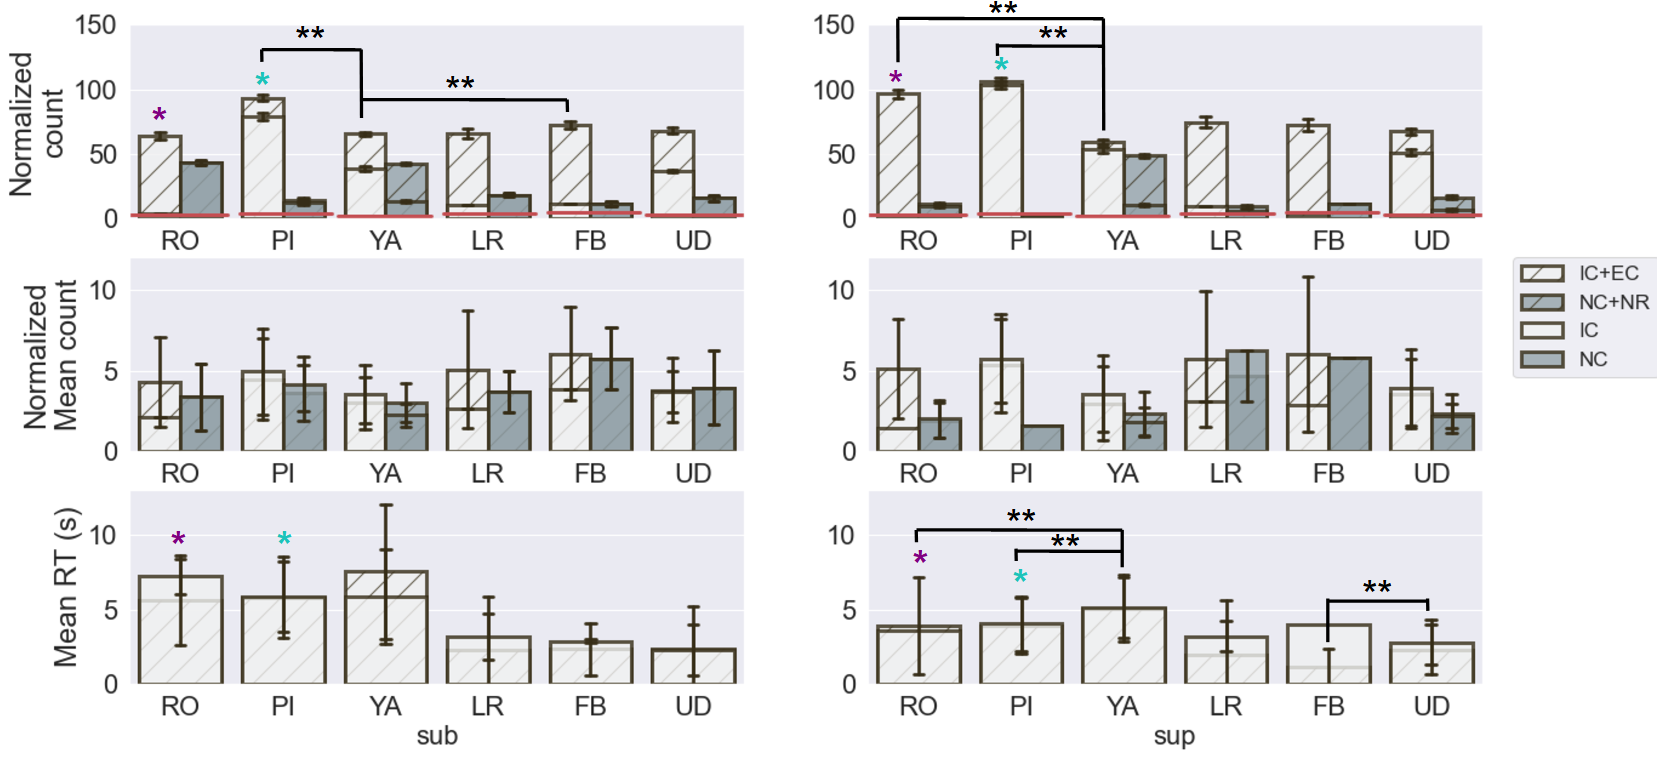
\includegraphics[width=0.9\linewidth]{Figure4_Final_count_TR_rot_trans_stars.png}
% \end{center}
% \caption{Normalized summed count (top row), normalized mean count (middle), and mean RT in seconds (bottom row) per detection performance profile for rotational and translational stimulation.  All 3 metrics (summed count, mean count, and mean RT) were compared for sub and sup speed stimulations for RO, PI, YA, LR, FB, and UD axes respectively; Wilcoxon signed rank test, and sum rank test were used to determine significance such that significant relationships were represented by (* within axis comparison of sub and sup, **: across axes comparison).  Bonferroni correction : p < 0.0167 was used as the significance threshold, p < 0.05 are mentioned as slight significant relationships.  Detection performance categories above the lower confidence interval, denoted by the solid red line, were considered for statistical comparison across subjects of categories within (ie: sub vs sup) and across axis (ie: RO sub vs PI sub) conditions.}
% \label{Figure4_Final_count_TR_rot_trans_stars}
% \end{figure}
% -------------------- 


\subsubsection{Detection: speed comparison (within axis condition)}
There was a slightly significant sub versus sup count difference for the most counted detection performance category for RO and PI axes, where sup speed resulted in a higher count than sub speed (RO count EC sup vs sub: Kolmogorov-Smirnov: nonnormal distribution, signedrank: p < 0.000244, sumrank: p < 0.026562, n=13; PI count IC sup vs sub: Kolmogorov-Smirnov: nonnormal distribution, signedrank: p < 0.081429 , sumrank: p < 0.201736, n=18).  The slight significance is denoted in the top row of Figure 4 with a single star in purple and blue.  There was a similar trend for the YA axis, where the most counted detection performance category IC had higher sup count in comparison to sub count.  This demonstrates that participants were more accurate during sup speed than sub speed, regardless of the motion stimulation axis or direction.  No significance between sub and sup speeds were found for the translational experiment.  However, there was a trend for all axes where the most counted detection performance category had higher sup count in comparison to sub count; refer to EC detection performance category for LR and FB axes and IC detection performance category for the UD axis.  Translational motion was less apparent than rotational motion, therefore we suspect that more data was needed in order for this trend to become statistically significance.

The fact that faster sup motion causes more accurate and faster motion detection than slower sub motion, is a result that has been reconfirmed in motion detection literature, thus confirming that the simulation experiment was performed correctly and the dataset accurately represents human response (\cite{Valko_2012_Vestibular}; \cite{Hartmann_2014_Direction}).  For the rotational experiment, some detection performance categories had significantly lower RT for sup than sub speed condition. For RO and PI axes, the RT for the most counted detection performance category was significantly lower for sup stimuli in comparison to sub speed (RO RT EC sup vs sub: Kolmogorov-Smirnov: nonnormal distribution, signedrank: p < 0.000184, sumrank: p < 0.000977, n=66; PI RT IC  sup vs sub: Kolmogorov-Smirnov: nonnormal distribution, signedrank: p < 3.88e-07, sumrank: p <  0.000004, n=65); significance is denoted in the bottom row of Figure 4 with a single star in purple and blue.

\subsubsection{Detection: axes comparisons (across axes per speed condition)}
The same speed condition and successful response categories denoted by IC and EC were compared across axes, in order to identify task difficulty with respect to axis and thus demonstrate that both experimental results were in alignment with psychophysical motion detection findings.  Whole-body motion detection literature shows that RO and PI are easier to detect than YA and translational motion; RO and PI detection thresholds were statistically similar for novices and experts (\cite{Hartmann_2014_Direction}).  Similarly, RO was easier to detect than LR, UD, and YA for both non-vestibular and vestibular dysfunction participants (\cite{Valko_2012_Vestibular}). 

For sup speed our dataset shows that successful response category counts for both RO and PI are significantly higher than counts for YA (sup PI count IC and EC vs sup YA count IC and EC: Kolmogorov-Smirnov: nonnormal, signedrank: p < 0.000002, sumrank: p < 0.004508, n=20; sup RO count IC and EC vs sup YA count IC and EC: Kolmogorov-Smirnov: nonnormal, signedrank: p < 0.000708, sumrank: p < 0.004158, n=20).  Additionally, for sub speed FB and PI had significantly higher counts than YA (sub YA count IC and EC vs sub FB count IC and EC: Kolmogorov-Smirnov: nonnormal, signedrank: p < 0.000213, sumrank: p < 0.008520, n=22; sub PI count IC and EC vs sub YA count IC and EC: Kolmogorov-Smirnov: nonnormal, signedrank: p < 0.000065, sumrank: p < 0.000355, n=22).  This shows that we similarly find that RO, PI and FB translational motion were easier to detect than YA, with dependence on speed when considering only correct responses.

Moreover, our results show functional differences between RO, LR, FB and PI, YA, UD tasks.  In PI participants mostly detected correctly (IC), and rarely when they did not detect correctly they eventually or never corrected.  In YA participants often detected correctly (IC), and sometimes when they did not detect correctly they did not feel any motion (NR).  In UD participants often detected correctly (IC),  and sometimes when they did not detect correctly they eventually corrected; IC was more prevalent when speed was fast.  Whereas in RO, LR, and FB, participants could not initially detect the correct axis and/or direction, but they could eventually find the correct axis after several mistakes.

Lastly, task difficulty for within rotational and translational stimulation appears to be correlated with longer RT.  For the rotational task at sup speed, RO and PI had faster RT than YA indicating that participants needed less time to detection motion for RO and PI (sup RO count IC and EC vs sup YA count IC and EC: Kolmogorov-Smirnov: nonnormal, signedrank: p < 4.31e-04, sumrank: p < 6.66e-06, n=67; sup PI count IC and EC vs sup YA count IC and EC: Kolmogorov-Smirnov: nonnormal, signedrank: p < 2.57e-04, sumrank: p < 7.09e-04, n=67).  Similarly, for the translational task at sup speed, FB had significantly faster RT than UD (sup FB count IC and EC vs sup UD count IC and EC: Kolmogorov-Smirnov: nonnormal, signedrank: p < 6.68e-04, sumrank: p < 9.73e-04, n=41).  Finally for completeness, for sup and sub speeds LR, FB, UD had significantly faster RT than RO, PI, and YA (nine 2-by-2 comparisons of each rotation and translation axis per sup and sub speed: Kolmogorov-Smirnov: nonnormal, signedrank :p < 5.6e-04, sumrank: p < 1.31e-03, n=45-67), because thresholds for rotational motion detection are lower than translational motion.  As mentioned in subsection 2.1.1 participants were stimulated slower in the rotational task than in the translational task thus RT should correspondingly be different and can not be compared.

\subsection{Participant detection performance rank}
Including both rotational and translational tasks, the highest rank score was 55 and the lowest score was 11.  On average, participants received a rank score of 37.  Therefore, the best performer, regardless of rotation or translation, achieved (55/72)*100=76.38% accuracy for the task.  And, the average performer was only able to achieve (37/72)*100=51.38% accuracy for the task.  The same task accuracy statistic was calculated for sub and sup conditions individually, for both rotation and translation experiments, and similar results were found shown in Table 1. 

Table 1: Experimental performance accuracy per speed condition using the rank performance measure.


These rank statistics shows that the detection task was challenging for the average person, regardless of the main speed condition (sub, sup) and the directional stimulation, however it was neither impossible to perform the task with reasonable success.  The participant distribution count for the Rotational experiment was: 5 best performers, 11 average performers, 2 worst performers. And, similarly, the participant distribution count for the Translational task was: 2 best performers, 11 average performers, 1 worst performers.  Based on the fact that the participant distribution count for best, average, and worst performance are similar for the rotational and translational task, this shows that both tasks were similarly challenging in terms of motion detection.  Therefore, translational detection may not more difficult than rotational detection in a realistic environment.


\subsection{Classification: SD prediction}
Classification accuracy was used to evaluate the predictive ability of each of the eight models; a value of 1 and 0 correspond to 100% and 0% correct prediction.  These accuracy results not only directly tell us which models are superior than others for given parameters, they also indirectly tell us about the data.  Figure 5 shows that decision tree type models (DT, GBC, RF) were superior to optimization based models (SGD, LDA, MLP, GNB, NuSVC) using the given features, regardless of the experiment type (rot, trans), axis, and speed.  Indirectly, this implies that important associations for SD prediction are not related to temporal or ordered information, because decision tree based models can not capture temporal patterns.  Additionaly, we trained models and tested both training and test hold-out data for both originally ordered features and reordered features with a gaussian distribution, accuracy results were similar for both analyses; gaussian distribution results are shown in Figure 5. The fact that prediction results were similar demonstrates that temporal ordering of movements were not an indicator for SD but rather the amplitude values. 

In comparing the three different semi-supervised labels, better accuracy can be obtained for optimization based models using a binary label in comparison to a multi-label (averaged lenient and strict vs complex:  Kolmogorov-Smirnov: nonnormal distribution, sumrank:p < 0.02, n=5).  In particular, the lenient label for the translational task produced higher accuracy for optimization based models (trans lenient vs complex: Kolmogorov-Smirnov: nonnormal distribution, sumrank:p < 0.0143, n=5).  However, regardless of the labels, there was no difference in accuracy for the decision tree based models. Indirectly, regarding optimization based models, this again indicates that SD and non-SD responses were similar.  Labeling with respect to correctness, the lenient label, better separates data with respect to amplitude than labeling based on initial correctness.

% -------------------- Figure 5 --------------------
% \begin{figure}[ht]
% \begin{center}
% 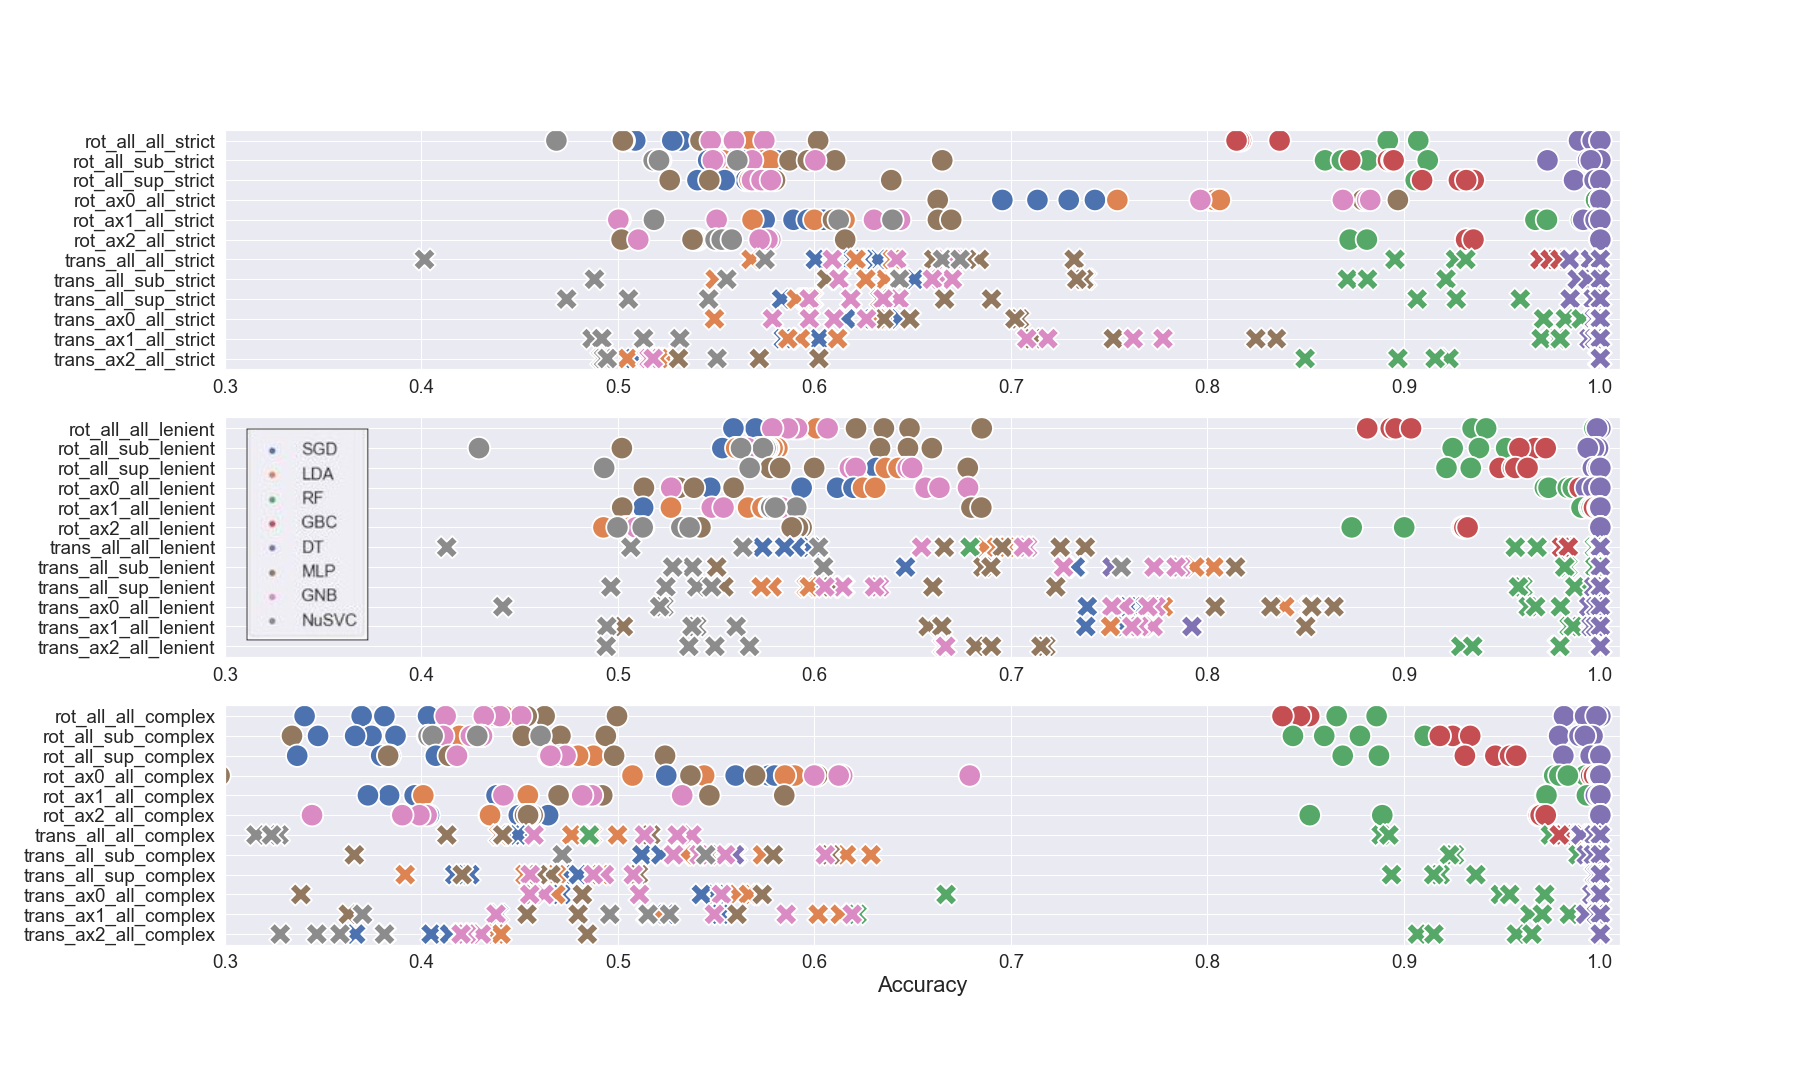
\includegraphics[width=0.9\linewidth]{Accuracy_comparisons_final_allfea_1.png}
% \end{center}
% \caption{Average 5-fold cross validation test prediction accuracy for the eight models for different: experimental data subsections, semi-supervised label (strict, lenient, complex), and number of features used.  For visual ease, circles and crosses correspond to the rotation and translation experiment types, respectively.  Blue, orange, green, red, purple, brown, magenta, and gray correspond to the SGD, LDA, RF, GBC, DT, MLP, GNB, and NuSVC models.  Regarding notation, ax0, ax1, ax2 indicate RO, PI, YA for the rotational task and LR, FB, UD for the translational task. Additionally, sup, sub, and all denote sup speed stimulation trials, sub speed stimulation trials, and all trials, respectively.}
% \label{Accuracy_comparisons_final_allfea_1}
% \end{figure}
% -------------------- 

Finally, we investigated whether modeling a subset of the data, such as an experimental axis or speed condition, would result in better prediction of SD for it’s use-case in comparison to predicting with a model built from combined use-cases.  Subset data models were trained and tested using data from specific experimental conditions, such as RO axis for both sub and sup speeds.  Subset data models were not tested on different experimental condition groups or use-cases, because model transferability was not of interest.  It was of interest to understand if specific use-cases needed their own individual models, or whether modeling combined use-cases was sufficient for predicting across use-cases on average.  Three dataset model test-prediction accuracy groups were compared using a non-parametric distribution test, for each of the three labels:  1) test prediction accuracy of models built from all the data, 2) averaged test prediction accuracy of models built from specific axis data, 3) averaged test prediction accuracy of models built from specific speed data.  No significant differences were found with regard to using all of the data in comparison to only speed or axis stimulus data, for decision tree models.  Optimization based models had four cases where there were accuracy difference with respect to the subset of data used.  Rotation axis data subset had higher accuracy for strict and complex than using all of the data (rot axis strict vs all data: Kolmogorov-Smirnov: nonnormal distribution, signedrank:p < 0.008, n=8 ; rot axis complex vs all data: Kolmogorov-Smirnov: nonnormal distribution, signedrank:p < 0.015, n=8).  There appears to be a predictive effect with using an initially correct label convention, strict or complex label, for axis condition data. Additionally, translational axis and speed data subset for the complex label had higher accuracy than using all of the data (trans speed complex vs all data: Kolmogorov-Smirnov: nonnormal distribution, signedrank:p < 0.02, n=8 ; trans axis complex vs all data: Kolmogorov-Smirnov: nonnormal distribution, signedrank:p < 0.05, n=8).  It is likely that using subset speed and axis data, instead of all of the data, helped to reduce variability such that distinguishing patterns could be found.

% -------------------- Figure 6 --------------------
% \begin{figure}[ht]
% \begin{center}
% 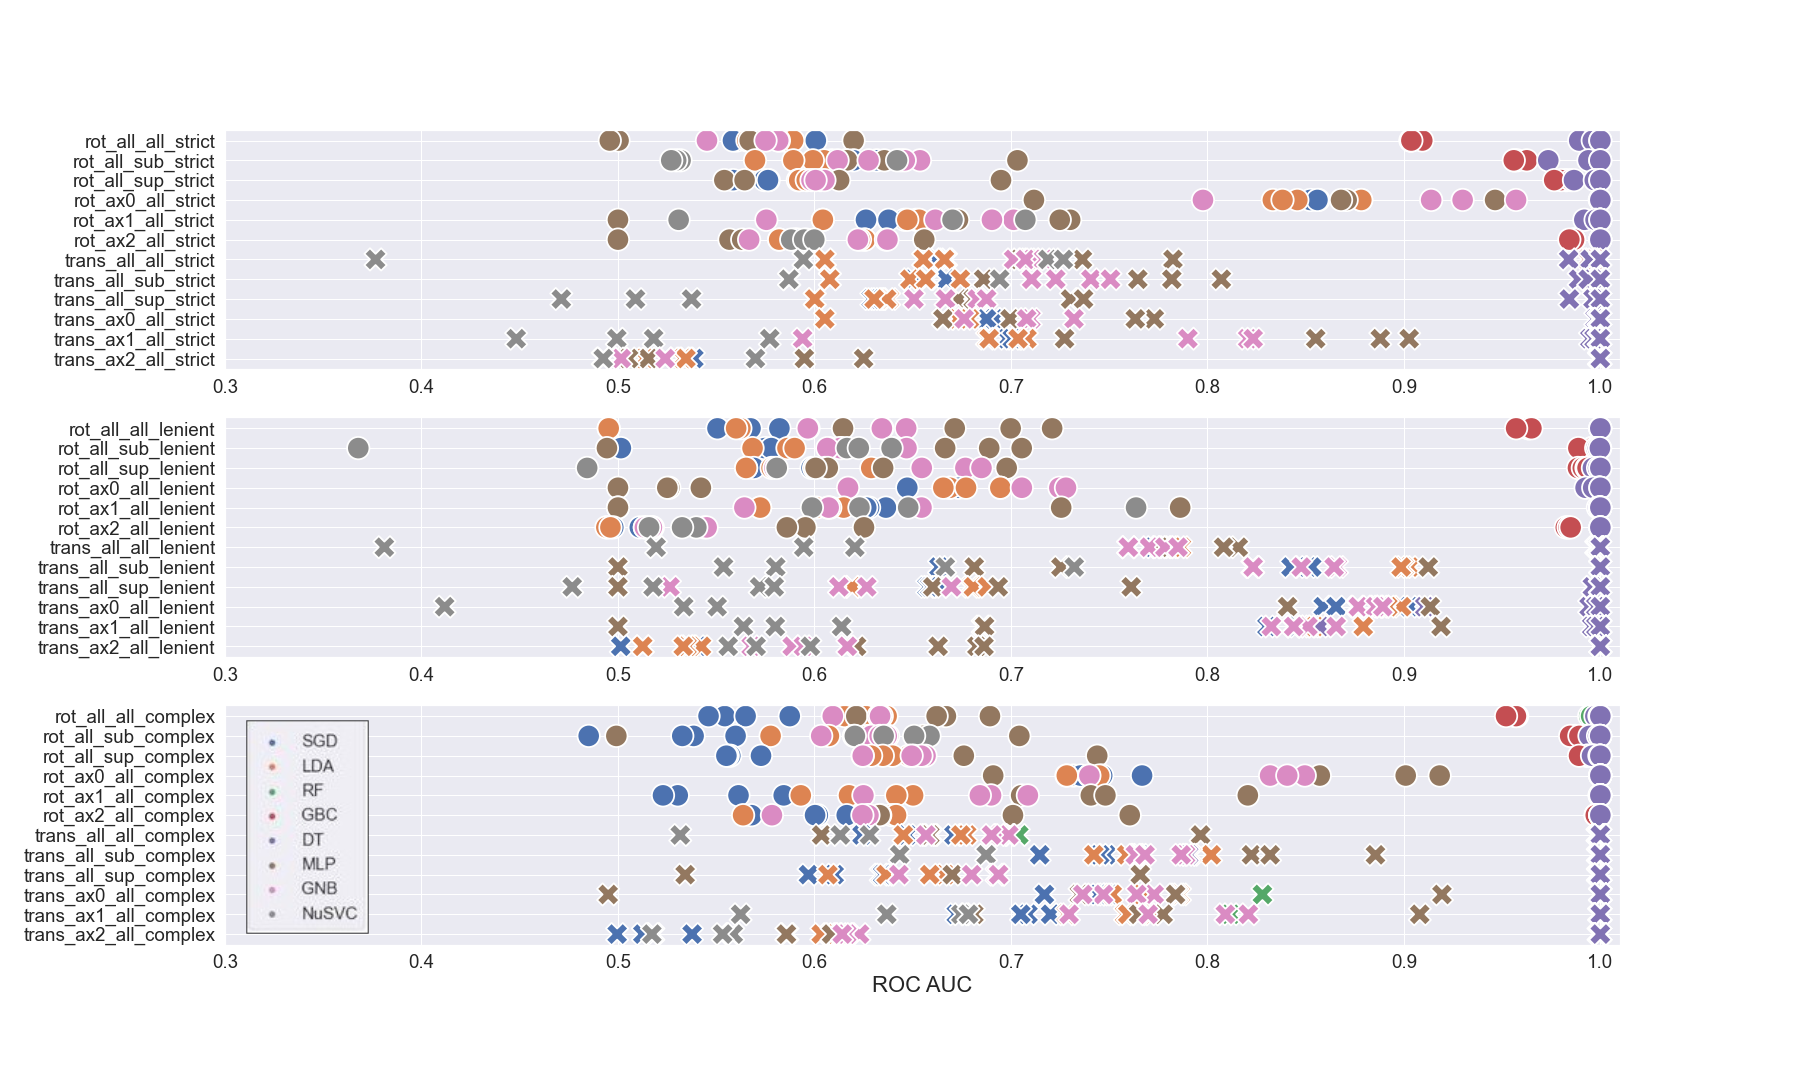
\includegraphics[width=0.9\linewidth]{ROCAUC_comparisons_final_allfea_1.png}
% \end{center}
% \caption{Test data ROC-AUC for the eight models for different experimental subsets of the data per semi-supervised label (strict, lenient, complex).  Circles and crosses correspond to the rotation and translation experiment types, respectively.  Blue, orange, green, red, purple, brown, magenta, and gray correspond to the SGD, LDA, RF, GBC, DT, MLP, GNB, and NuSVC models.  Regarding notation, ax0, ax1, ax2 indicate RO, PI, YA for the rotational task and LR, FB, UD for the translational task. Similarly, sup, sub, and all denote sup speed stimulation trials, sub speed stimulation trials, and all trials, respectively.}
% \label{ROCAUC_comparisons_final_allfea_1}
% \end{figure}
% -------------------- 

The Receiver Operating Characteristic Area Under the Curve (ROC-AUC) measure, shown in Figure 6, was used to evaluate the model's predictive ability with respect to the label value, to evaluate whether the models could predict correctly regardless of the label value.  Figure 6 shows the same three main results as the accuracy results, indicating that the models are reliable in terms of identifying SD and non-SD data, and thus the accuracy value based on true positive and negative counts can be trusted.  The 3 summarized main results were: 1) decision tree type models (DT, GBC, RF) have almost perfect prediction and the majority of optimization based models (SGD, LDA, MLP, GNB, NuSVC) have above chance level prediction regardless of the class label value (averaged lenient and strict vs complex:  Kolmogorov-Smirnov: nonnormal distribution, sumrank:p < 0.02, n=5). 2) Decision tree models predict well regardless of initial correctness or overall correctness label usage, however optimization based models predict best when labels are constructed with respect to overall correctness via the lenient label (trans lenient vs complex: Kolmogorov-Smirnov: nonnormal distribution, sumrank:p < 0.027, n=5).  3) Models using all of the data instead of a subset of the data, provided similarly accurate performing models except for 4 cases.  Rotation axis data subset had higher accuracy for strict and complex compared with using all of the data (rot axis strict vs all data: Kolmogorov-Smirnov: nonnormal distribution, signedrank:p < 0.05, n=8 ; rot axis complex vs all data: Kolmogorov-Smirnov: nonnormal distribution, signedrank:p < 0.015, n=8).  Translational axis and speed data subset for the complex label had higher accuracy in comparison to using all of the data  (trans speed complex vs all data: Kolmogorov-Smirnov: nonnormal distribution, signedrank:p < 0.02, n=8; trans axis complex vs all data: Kolmogorov-Smirnov: nonnormal distribution, signedrank:p < 0.05, n=8).

% -------------------- Figure 7 --------------------
% \begin{figure}[ht]
% \begin{center}
% 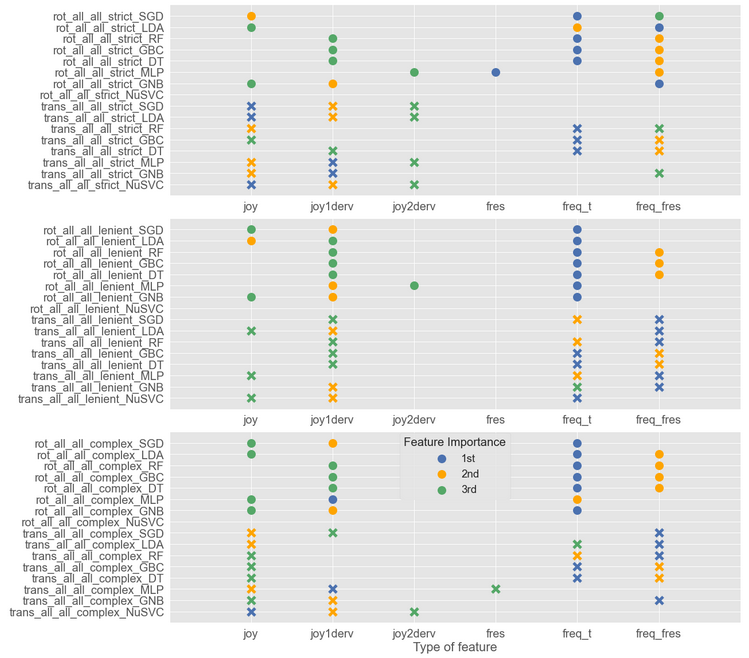
\includegraphics[width=0.9\linewidth]{Feature_comparisons_final_matplotlib.png}
% \end{center}
% \caption{Feature order importance based on permutation importance, for each model.  Blue, orange and green circles indicate most important feature, second most important feature, and third most important feature.}
% \label{Feature_comparisons_final_matplotlib}
% \end{figure}
% -------------------- 

Feature order importance allows for us to know which aspect of the joystick signal contains key information to detect spatial disorientation.  Figure 7 shows the feature importance for models where all the rotational or translational data was used.  Three main findings were identified: 1) decision tree models perform optimally using extracted temporal information constant features, 2) optimization based model feature importance identified more temporal features as being important than constant features, 3) semi-supervised labels did not influence feature importance for decision tree models however the strict label for optimization based models identified only temporal features as being important.

Extracted temporal information, such as the signal's natural frequency, that was transformed into a constant scalar feature greatly improved decision tree model prediction accuracy.  Regardless of the semi-supervised label type and experiment, decision tree models relied on natural frequency based features, more than position based features, to predict SD.  It is likely that these models found stronger patterns with natural frequency features because these feature values repeat per trial, instead of having a unique temporal trace like position based and the frequency response features. Decision tree model prediction accuracy was tested only using the four temporal features, and accuracy results were substantially less accurate at an average of 0.7 in comparison to 0.9 when the two natural frequency constant features were included.  Decision tree models are good at finding recurring/mode-like patterns between the features and the corresponding labels, whereas the optimization models are good at finding recurring patterns coupled with specific constraints such as causality.  In general, feature importance for decision tree models, from most to least important, were: 1) constant natural frequency of the joystick signal using a periodic estimation method, 2) constant natural frequency of the joystick signal using a frequency response method, and 3) the derivative of the joystick signal.  Optimization based models where shown to be more sensitive to temporal features than the decision tree models, where more temporal features were identified to be more important than constant natural frequency features.  By average, feature importance for optimization based models, from most to least important, were: 1) constant natural frequency of the joystick signal using periodic estimation, 2) the derivative of the joystick signal, 3) the joystick signal.

\subsection{Perceived motion and physical disorientation}
Twenty of the 31 total participants did not feel any difference in terms of physical disorientation over the entire experiment.  Considering, the performance rank score mentioned in 4.2, roughly 1/3 of average detectors, 1/3 of best detectors, and 2/3 of worst detectors felt physical disorientation.  The 2/3 worst detection ratio is reported for completeness, however this measure is disregarded because it is based only on 3 participants.  Thus, 1/3 of the population regardless of performance felt physical disorientation.

To investigate whether there was a relationship between physical disorientation and detection performance, detection performance for the 12 participants who reported physical disorientation was evaluated; see Table 2 for a percentage of their summed trial performance per category per SSQ difference report.  For instance, a participant who reported a 6 after the experiment and a 4 before the experiment would have their trial performance categories (ie : 8 trials were category 2, 6 trials were category 1, etc) associated with the SSQ score of -2.  Table 2 demonstrates that more negative physical disorientation was observed for unsuccessful initial detection response profiles (EC and NC) than for IC successful initial detection response or no response. The negative and positive SSQ disorientation differences per response category were summed respectively, to evaluate significance between IC negative and NC or EC negative.  Physically disoriented good performers (IC) did not report significantly less physical disorientation than poor performers.


Table 2: Occurrence response category per reported SSQ disorientation subscale difference, for both rotational and translational experiments.  The bold negative SSQ values for categories EC and NC highlight that more negative physical disorientation was present for unsuccessful initial attempts to detect motion.

In summary, we report no significant relationship between physical disorientation and motion detection.  There is only a trend that EC and NC performers, that felt physical disorientation, felt better before the task than after.  Implying that participants became fatigued while trying to perform the task, when detection was not easy for them.  For IC performers that felt physical disorientation, there was no trend in terms of feeling better before or after.  Implying that participants who could detect easily, felt discomfort for other reasons not related to the experiment.  There was a slight trend for NR performers that felt physical disorientation, such that they felt better after the task than before.  Showing that participants who did not respond, became comfortable and relaxed in the dark experimental setting.


\section{Discussion}
In this comprehensive study about spatial disorientation, we demonstrate that it is possible to isolate, simulate, and recreate realistic aspects of a vestibular feedback piloting task and predict the occurrence of spatial disorientation using joystick response as a feature.  The experimental design allowed for the collection of perceptual response joystick data during various basic scenarios of vestibular and proprioceptive stimulation such that depending on the joystick response, SD or non-SD was apparent.  A crucial data standardization step was used to verify that the simulator system performed the experimental design correctly, removing trials with delays and erroneous motion.  This SD-targeted dataset captures known human motion perception trends, demonstrating that the dataset reliably captures motion detection behavior.  Known motion detection trends include : a) accurate and faster response for supra speed stimulation in comparison to near sub-threshold speed stimulation, b) PI, RO, FB, LR, UD, and YA were the least to most difficult axes tasks, c) longer reaction times corresponded with task difficulty for respective rotational and translational experiments (\cite{Valko_2012_Vestibular}; \cite{Hartmann_2014_Direction}; \cite{Karmali_2017_Multivariate}).  Ranking of task difficulty per axis confirms literature reports that there is no sensory advantage for UD detection due to gravity, because the vestibular system compensates for gravity (\cite{Valko_2012_Vestibular}).  In addition to confirming known motion detection trends, functional differences in motion detection for RO, LR, FB and PI, YA, UD tasks were observed; where the most counted response for RO, LR, FB was EC in comparison to IC for PI, YA, UD.  It is unclear why participants made more initial mistakes for  RO, LR, and FB than PI,YA, and UD axes, however perhaps participants relied on more non-vestibular sensory cues (proprioception, tactile, auditory from the simulator motor) and/or had better natural upright posture during certain stimulus motions than others.  Perhaps in PI, YA, and UD they relied more upon clear vestibular cues because they self-generated less additional motion information from self-motion or joystick interaction, thus allowing participants to either initially detect correctly or not.  It appears plausible that in RO, LR, and FB participants were more likely to generate additional and perhaps conflicting sensory information by naturally tilting or turning the head.  It is likely that participants naturally adapted their posture, to be more or less upright, during certain motion stimuli in comparison to others.  For example, a slightly left tilted head during pitch motion would more likely induce discomfort than during roll motion, thus encouraging participants to naturally sit upright during pitch stimuli and thus giving them an advantage to detect the motion more clearly.  Such functional errors in RO, LR, and FB caused by natural postural behavior could easily escalate the occurrence of spatial disorientation.

Statistical analysis showed that regardless of experimental conditions the best performers achieved 76% detection accuracy and average performers achieved $51\%$ accuracy.  The task may have been difficult because participants were given the freedom to decide on which axis and in what direction the stimulation occured, as is done in a real-life piloting situation.  All participants had very little to no piloting experience, thus our results reflect human motion perception without the influence of piloting experience or training.  Thus, the modeling results obtained from this dataset may not be representative of expert piloting behavior,  because our novice participant response's have more variability than expert piloting responses.

Using the SD dataset we investigated modeling methods to predict SD, including statistical analysis, predictive control, and machine learning.  Predictive control has been used to predict motion detection (\cite{Soyka_2011_Predicting}), however ML methods have been shown to be efficient and accurate at finding patterns amongst different types of data and constructing reusable models for future prediction (\cite{Burkov_2019_ML}).  Using ML techniques, we investigated how to optimally predict SD and explain the importance of different parameter selections.  We evaluated the importance of model construction parameters by using test set prediction accuracy and ROC-AUC as a benchmark and comparative measure.  Five key model construction parameters were tested: number of features, 8 model types, dataset conditions, feature type, semi-supervised label type.

Regarding the number of features in each ML model, no significant difference were found in prediction accuracy when using all six joystick features, three of the most important features, two of the most important features, or the most important feature alone. Thus, building a model on a single important feature is sufficient to predict SD.  However, it is a best practice to use all relevant features for model construction.

Decision tree type models (DT, GBC, RF) were superior, to optimization based models (SGD, LDA, MLP, GNB, NuSVC), in test accuracy prediction regardless of the experiment (rot, trans), axis, speed, and semi-supervised label.  On average decision tree models had accuracy rates ranging from 0.8-0.99 depending on the model type.  These models were able to learn associations between the features and the label regardless of semi-supervised label construction.  However, optimization based models predicted best when labels were constructed with a binary label instead of a multi-label.  More specifically, the lenient label resulted in better prediction than the strict label.  On average optimization based models with binary labels had accuracy rates ranging from 0.5-0.85. 

Specialized models for axis or speed conditions did not outperform models where all the data was used for decision tree models.  Whereas, for optimization based models, for optimization based models, some specialized models predicted better using a complex multi-label predicted better than average prediction of models where all the data was used.  This shows that if the feature patterns are difficult to organize using specific ML optimization strategies, semi-supervised label selection is crucial in highlighting distinguishing feature patterns.  A label with many classes needs data with less variability such that each class can be distinguishable from the other.

Three main findings were identified during feature importance investigation: 1) decision tree models perform best using constant natural frequency features, 2) optimization based model feature importance identified more temporal features as being important than constant natural frequency features, 3) semi-supervised labels did not influence feature importance for decision tree models however the strict label for optimization based models identified only temporal features as being important.  When an ML model performs poorly or does not select a feature as being important, it means that the optimization strategy can not produce a prediction in alignment with the label, using the given feature information.  Optimization based models poorly use features with repeating constant values because the optimization strategies often require feature data point distances to be optimized in a certain manner. Feature data points with the same value do not allow for the optimization algorithms to find optimal maximization or minimization predictions.  In hindsight, instead of using constant natural frequency features it would be more beneficial for optimization methods, to create a more complex natural frequency feature using wavelets or PCA, or a feature created from a clustering method like kmeans.  Despite the fact that decision tree models appear to be more accurate and easier to tune than optimization based models, optimization based models are useful for data with stationarity and merit the additional time to optimally tune these models.  An optimally-tuned optimization based model would be able to predict the occurrence of SD while accounting for stationarity trends, like those that occur during the leans SD use-case, while decision tree models are more likely to confuse the trend with SD related behavior. 

Finally, the decision to choose a strict or complex label convention versus a lenient label to discern SD depends on the application and the quantity of data available to represent a non-SD state.  The strict label was less realistically representative of non-SD, because perfect behavioral data in any task is statistically rare, thus building an accurate model using a strict label convention maybe more challenging. Similarly, for the complex semi-supervised label there was lack of representative data for each of the SD cases.  Over-fitting, where training predictions were higher than test predictions, was observed for both strict and complex labels supporting a lack of data for these labeling conventions.  The lenient label, labeling with respect to overall correctness regardless if mistakes are made, was shown to be the best labeling convention as: 1) over-fitting was less observed for our small dataset where test and training predictions were similar, 2) both natural frequency and temporal features were selected as important features thus a diversity of relevant simple patterns were captured.  Moreover, prediction accuracy with respect to semi-supervised label construction can be used as a confirmation for how to define SD because semi-supervised means that the label is not 100% the ground truth.  The prediction accuracy of the model construct using the data, conveys the missing information about the label based on trends in the data. If a model predicts better with label A than label B it means that label A better matched the existing data structure, thus confirming that label A is likely to be the ideal label for the data.  Therefore, applying this idea to the three semi-supervised SD labels.  The lenient label is the ideal label convention for modeling SD, with respect to our dataset, because on average both decision tree and optimization based models predicted the test data best using the lenient.  A lenient label convention, where SD is defined as never correct or no response, is also in alignment with the definition of SD, where SD is defined as involving successive failures and major performance error (\cite{Newman_2007_SD}).

One-third of participants felt physical disorientation during the task, however no significant relationship between physical disorientation and motion detection was found.  There was a trend where participants who initially detected unsuccessfully felt worst after the experiment than participants who did initially detected successfully or did not try.  More sample points regarding physical disorientation are needed during the experiment, instead of a sample before and after the task, in order to determine if physical disorientation is correlated with motion detection.  Based on our results, questionnaire methods for ascertaining information about physical disorientation are insufficient to uncover correlations with perceptual disorientation.  A physiological sampling measure that implies physical discomfort, with a comparable sampling rate as the joystick such as EEG, NIRS, heart rate, or electrodermal activity could provide more insight into correlations with physical and perceptual disorientation.


\newpage
% -----------------------------------------
% References
% -----------------------------------------
\bibliography{bib}
\nocite{*}


% \newpage
% \section*{Biographies}
% For each author, indicate the current affiliation and highest degree obtained (field, year obtained, institution)

\end{document}